The main motivation which leads us to look for another approach to be used is that we want to:
\begin{enumerate}
    \itemsep0em
    \item Use a small amount of data
    \item Have \textit{mild} assumptions on the noise.
\end{enumerate}

\section{Main ingredients}
In order to formulate the \textbf{Set-Membership System Identification problem} we need some important ingredient:
\begin{itemize}
    \itemsep0em
    \item We start from a discrete time \textit{parametrized regression form} 
    \begin{equation*}
        y(k) = f(y(k-1),...,y(k-n), u(k), u(k-1), u(k-m), \theta_1, ..., \theta_{n+m+1}), \quad m \le n
    \end{equation*}
    \item A-priori assumptions on the \textbf{system} $\mathcal{S}$:
    \begin{itemize}
        \item $m,n$ are known; 
        \item The function $f\in\mathcal{F}$ (for the moment we choose the LTI class of dynamical systems).
    \end{itemize}
    \item A-priori assumptions on the \textbf{noise}:
    \begin{itemize}
        \item Noise structure (\textbf{OE, EIV}); 
        \item The input and output noise is part of some \textbf{bounded sets} $\mathcal{B}$ and in particular:
        {\large{
            \begin{align*}
                &\eta(k)\in\mathcal{B}_\eta, \quad
                \xi(k) \in \mathcal{B}_\xi
            \end{align*}
        }}
    \end{itemize}
    Tipically the sets $\mathcal{B}$ are defined by \textbf{polynomial constraints}, it is common that
    {\large{
        \begin{equation*}
            \mathcal{B}_\eta = \{
                \eta: \ \vert \eta(k) \vert \le \Delta\eta
            \}, \quad
            \mathcal{B}_\xi = \{
                \xi : \ \vert \xi(k) \vert \le \Delta\xi
            \}
        \end{equation*}
    }}
\end{itemize}

The \textbf{key element} of the Set-Membership identification method is the research of the \textbf{Feasible parameter set (FPS)} that we denote with $\mathcal{D}_\theta$. In a nutshell, it is the set of the parameter $\theta$ such that all the conditions exposed are fullfilled.

\section{Noise structures}

\subsection{Error-In-Variable set-up (EIV)}
\begin{figure}[h]
    \centering 
    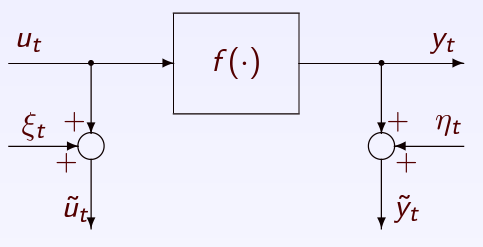
\includegraphics[scale=1]{images/EIV.png}
    \caption{EIV set-up}
\end{figure}
\textbf{Error-In-Variables (EIV)} problem refers to the most general case where the measurement noise is added both in the input and the output.\\
Due to the conditions we mentioned, we  have that:
{\large{
    \begin{equation*}
        \xi = [\xi(1) \quad ... \quad \xi(H)]\in \mathcal{B}_\xi, \quad
        \eta = [\eta(1) \quad ... \quad \eta(H)]\in \mathcal{B}_\eta
    \end{equation*}
}}

\subsection{Output-Error set-up(OE)}
\textbf{Output-Error(OE)} problem arises when the measurement noise $\eta$ enters only on the output of the system, while the system is assumed to be \textbf{exactly known}. [This is not strange to assume because sometimes one build the sequence of input to stimulate the system]. \\
Due to the condition we mentioned, we have that:
{\large{
    \begin{equation*}
        \eta = [\eta(1) \quad ... \quad \eta(H)]\in\mathcal{B}_\eta
    \end{equation*}
}}
\begin{figure}[h]
    \centering
    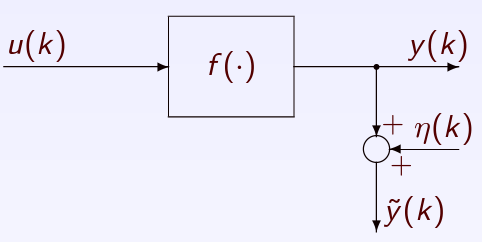
\includegraphics[scale=1]{images/OE.png}
    \caption{OE set-up}
\end{figure}

\section{Feasible Parameter Set (FPS)}
In the framework of \textbf{Set-Membership(SM) Identification}, all the parameters values consistent with the (i) \textit{a-priori information on the model}, (ii) \textit{a-priori information on the noise}, (iii) collected input/output data are considered as:
\begin{center}
    \large
    Feasible solution of the system identification problem
\end{center}
The set of all the parameters which satisfies these conditions is called the \textbf{Feasible Parameter Set}. For a \textbf{general EIV problem} it can be implicitly defined as:\\

\hspace*{-5mm}
\begin{tikzpicture}
\node [mybox] (box){%
    \begin{minipage}{.96\textwidth}    
        {\normalsize{
            \textbf{Feasible Parameter Set (FPS)}\\
    \begin{equation}
        \begin{aligned} \label{eq:FPS}
            \mathcal{D}_\theta = &\{
        \theta\in\mathbb{R}^p: \
        y(k)=f(y(k-1), ..., y(k-n), u(k),u(k-1), ..., u(k-m), \theta),\\
        & k=n+1,...,H,\\
        & y(k)=\tilde{y}(k)-\eta(k), \quad 
        u(k)=\tilde{u}(k)-\xi(k), \ k=1, ..., H\\
        &\vert \xi(k) \vert \le \Delta\xi, \ 
        \vert \eta(k) \vert \le \Delta\eta, \ 
        k=1,...,H
        \}
        \end{aligned}
    \end{equation}
}}
    \end{minipage}
};
\end{tikzpicture}%

\noindent
In the case that we want to identify a LTI discrete time system the set (\ref{eq:FPS}) is:
{\large{
    \begin{equation}
        \begin{aligned}
            \mathcal{D}_\theta =&\{
                \theta\in\mathbb{R}^p: \ 
                (\tilde{y}(k)-\eta(k))+
                \sum_{i=1}^n {\theta_i (\tilde{y}(k-1)-\eta(k-1))} =\\ &=\sum_{j=0}^m {\theta_j} (u(k-j)-\xi(k-j)), \ k=n+1, ..., H \\
                &\vert \xi(k) \vert \le \Delta\xi, \ 
                \vert \eta(k) \vert \le \Delta\eta, \ 
                k=1,...,H
            \}
        \end{aligned}
    \end{equation}    
}}

\noindent
The \textit{Feasible Parameter Set} enjoys the following properties:
\begin{enumerate}
    \itemsep0em
    \item The \textit{true value} of the parameter vector $\theta$ is guaranteed to belong to $\mathcal{D}_\theta$; 
    \item $\mathcal{D}_\theta$ implicitly quantify the uncertainty affecting the found mathematical model.
\end{enumerate}

Once we have found the FPS, we can use it to find \textbf{for each parameter} $\theta_k$ the \textit{Parameter Uncertainty Interval (PUI)} which is formally defined as
{\large{
    \begin{align}
            &PUI_k = [\underline{\theta}_k;\ \overline{\theta}_k], \\
        &\underline{\theta}_k=\min_{\theta\in\mathcal{D}_\theta} {\theta_k}, \quad \overline{\theta}=\max_{\theta\in\mathcal{D}_\theta} {\theta_k} \label{eq:PUIs}
    \end{align}
}}
The computation of $PUI_k$ requires to compute the \textbf{global optimal solution} of the optimization problems in (\ref{eq:PUIs}).

\subsection{Example \#1}
Let us suppose that the model to identify is a static system: a resistor.

\subsubsection{Ingredients}
\begin{enumerate}
    \item \textsc{A-priori information on the system}: $y(k)=\theta u(k)$
    \item \textsc{A-priori information on the noise} here we assume a \textbf{OE} noise structure, where $\vert \eta(k) \vert \le \Delta\eta$
    \item \textsc{A-posteriori info (I/O collected data)}, I have the pairs $[u(k), \tilde{y}(k)], k=1,...,H$
\end{enumerate}

\subsubsection{Feasible Parameter Set Computation}
{\large{
    \begin{align*}
        &\begin{aligned}
            \mathcal{D}_\theta = &\{
                \theta \in \mathbb{R}: y(k)=\theta u(k) \forall k=1,..., H \\
                &y(k)=\tilde{y}(k)-\eta(k), \quad \forall k=1,...,H\\
                &\vert \eta(k) \vert \le \Delta\eta
            \}\Longleftrightarrow
        \end{aligned}\\ 
        &\begin{aligned}
            \mathcal{D}_\theta = &\{
                \theta \in \mathbb{R}: \tilde{y}(k)-\eta(k)=\theta u(k), \quad
                \vert \eta(k) \vert \le \Delta\eta, \ 
                k=1,...,H 
            \}
        \end{aligned}\\
        &\begin{aligned}
            \mathcal{D}_\theta = &\{
                \theta \in \mathbb{R}: \eta(k)=\tilde{y}(k)-\theta u(k), \quad
                \vert \eta(k) \vert \le \Delta\eta, \ 
                k=1,...,H 
            \}
        \end{aligned}\\
        &\begin{aligned}
            \mathcal{D}_\theta = \{
                \theta \in \mathbb{R}: \
                -\Delta\eta \le \tilde{y}(k)-\theta u(k) \le \Delta\eta, \quad
                k=1,...,H
            \}
        \end{aligned}\\
        &\begin{aligned}
            \mathcal{D}_\theta = \bigg\{
                \theta \in \mathbb{R}: \ 
                \theta \ge \frac{\tilde{y}(k)-\Delta\eta}{u(k)}, \ \theta \le \frac{\tilde{y}(k)+\Delta\eta}{u(k)}, \quad \forall k=1,...,H
            \bigg\}
        \end{aligned}
    \end{align*}
}}
In this case the FPS is the intersection between $H$ intervals, and the $PUI$ for the only parameter $\theta$ is coincident with this found interval.
We succeded in eliminating the dependence on $\xi,\eta$, but this was a particular case.\\
If only the system to identify had been only a little bit more complicated, the trick we used to eliminate $\eta$ from the set, would not have work. 

\section{Extended Feasible Parameter Set (EFPS)}
\noindent
This fact highlight the necessity to enlarge the FPS in such a way, it is able to contain also the variable $\theta, \xi$ which depends on the input and output error, defining the \textbf{Extended Feasible Parameter Set (EFPS)}.\\

\hspace*{-5mm}
\begin{tikzpicture}
\node [mybox] (box){%
    \begin{minipage}{.96\textwidth}     %Larghezza del box
        {\normalsize{
            \textbf{Extended feasible parameter set (EFPS)}\\
            \begin{equation}
                \begin{aligned}
                    \mathcal{D}_{\theta,\xi,\eta} =&\big\{
                        \theta\in\mathbb{R}^p,\ 
                        \xi \in \mathbb{R}^H, \
                        \eta \in \mathbb{R}^H: \ 
                        (\tilde{y}(k)-\eta(k))+ 
                        \sum_{i=1}^n {\theta_i (\tilde{y}(k-1)-\eta(k-1))} =\\ &=\sum_{j=0}^m {\theta_j} (u(k-j)-\xi(k-j)), \ k=n+1, ..., H \\
                        &\vert \xi(k) \vert \le \Delta\xi, \ 
                        \vert \eta(k) \vert \le \Delta\eta, \ 
                        k=1,...,H
                    \big\}
                \end{aligned}
            \end{equation} 
        }}
    \end{minipage}
};
\end{tikzpicture}%

This is the set of the parameters $\theta$ and noise samples $\xi, \eta$ which are consistent with the \textit{a-priori assumptions}. The FPS $\mathcal{D}_\theta$ we defined in the previous paragraphs is only the projection in the parameter space $\mathbb{R}^p$ of the EFPS $\mathcal{D}_{\theta,\xi,\eta}$.
Moreover the PUIs have to be computed on the extended space that in general is a \textbf{non-convex set} defined by \textbf{polynomial constraints}, in the following way:
{\large{
    \begin{equation}
        \underline{\theta}_k=\min_
        {\theta,\xi,\eta\in\mathcal{D_{\theta,\xi,\eta}}} {\theta_k}, \quad \overline{\theta}=\max_{\theta,\xi,\eta\in\mathcal{D_{\theta,\xi,\eta}}} {\theta_k} \label{eq:PUIs}
    \end{equation}
}}
One can wonder how to use the PUI for each parameter once you found it.  Usually for each $PUI_k$, the best choice is the \textbf{central estimate} $\theta_c$ defined as
\begin{equation*}
    \theta_{c,k} = \frac{\underline{\theta}_k+\overline{\theta}_k}{2}
\end{equation*}
This is the value which minimizes the uncertainty on the parameters.

\section{Convex relaxation for PUIs computation}


 







